\documentclass{article}
\usepackage[english]{babel}
\usepackage[utf8]{inputenc}
\usepackage{fancyhdr}
\usepackage[hidelinks]{hyperref}
\usepackage{graphicx}
\usepackage{subcaption}
\usepackage[inline]{enumitem}
\usepackage[a4paper, margin=1in]{geometry}

\makeatletter
\newcommand\footnoteref[1]{\protected@xdef\@thefnmark{\ref{#1}}\@footnotemark}
\makeatother

\newcommand{\question}[1]{\section{#1}}
\pagestyle{fancy}
\fancyhf{}
\rhead{Question \thesection}
\lhead{Elliot Greenwood and Jonathan King}
\lfoot{Continuous Delivery}
\rfoot{Page \thepage}

\begin{document}

\question{What are the problems that a build pipeline is trying to solve?}
A build pipeline is a linked set of stages that represent the process of releasing a new feature (or bug fix etc.) into production.
These stages are usually along the lines of:
\begin{itemize*}
  \item fetching dependencies
  \item building the patch against the master branch/trunk
  \item running automated test suites
  \item bundling artefacts
  \item deploying to a staging environment
  \item deploying to a production environment
\end{itemize*}.
Build pipelines are beneficial because these stages can be run automatically as soon as the preceding step has completed,
or manually or at a set time of the day.
It completely depends on what your company/team wants to do, affording you great flexibility in your process.
Within each stage you can have multiple steps that can run in parallel,
for example unit tests, feature tests and integration tests can all run at the same time.
This can dramatically reduce the time of your builds.
You also have some guarantees that each build is reliable and reproducible,
meaning you spend less time every release cycle fixing issues with broken builds.
This is more likely to encourage more frequent releases (or more frequent merges, if the releases are not instant).
\par
There are numerous tools and services that provide methods for doing all of this for you.
You build pipeline could be an all in one solution such as Gitlab CI\footnote{\label{gitlab-ci}} or Jenkins\footnote{\label{jenkins}},
or one that stretches across many services (perhaps using Github\footnote{\label{github}}, Team City\footnote{\label{team-city}} for building and Octopus\footnote{\label{octopus}} for deployment).
All of these tools have different methods of specifying what happens during the build.
Some systems use an Infrastructure as Code style technique (Jenkins\footnoteref{jenkins}),
others use graphical layouts (Team City\footnoteref{team-city} and Gitlab CI\footnoteref{gitlab-ci}),
simpler systems such as Travis\footnote{} and Circle CI\footnote{} use simple config files.
\par
Using these tools and services boasts many benefits such as cached dependencies,
for example in our build pipeline (Page 2) we use Travis to build and we are able to cache the core latex packages we would otherwise need to download.
This caching can speed up the times of our builds, we were able to reduce our time down from 6 minutes to approximately 2 minutes.
Additionally, it means that if somebody releases a new version of the \texttt{hyperref} package that has deprecated the \texttt{hidelinks}
option that we use our cached versions will continue to be used, ensuring our build won't start passively failing.
You can imagine in a more real world example this could be a npm package or something similar,
where there are many packages that can take some time to download and install.
\par
Ideally after the build process has been completed you should have everything you need to deploy the newest version of your software~\cite{BruntonBuild}.
This means that as much as possible, you include everything needed for the final host machine to run the application.
Or this can mean bundled packages ready to be uploaded to a private npm server.
In his blog post~\cite{BruntonBuild} Brunton-Spall comments on this and describes
how if you are extremely unlucky you can have changes between testing and deploying if your artefacts are not immutable.
\par
If the builds are successful and the tests pass you can deploy to some staging servers you may have for internal testing, demoing or focus group testing etc.
This means even if you only release to master once per week, say,
you have somewhere that gives you an indication of what it will be like in production,
and also whether or not anything appears to have broken that slipped through the testing-net.
\par
Due to the fact build pipelines offer reproducible builds you can deploy to multiple clients with ease and in parallel,
by simply defining the configuration for the build in each case.
%%%%%%%%%%%
% The main problems that having a build pipeline addresses are automation and ease of delivery.
% For anything much larger than a toy project you will likely want a script to run various tests,
% perhaps one command for all suites, another for just unit tests etc. but running lots of scripts can become a pain.
% Continuous Integration (CI) tools can do away with many of these scripts by providing a user friendly way of setting up a build pipeline that automates lots of common tasks.
% Automating the fetching of dependencies, building the product, running various stages of tests, and collecting all of the artefacts that are produced can save developers a lot of time.
% By saving developers a lot of time it will encourage developers to make releases more often,
% perhaps with features turned off until the business is ready or another service has been updated.
% Having an automated build server can also provide performance benefits.
% Many services, such as Travis CI, have dedicated, specialised servers for building projects in parallel,
% as well as caching specific versions of dependencies,
% this means if new releases become available your build will not break.
% \par
% Most continuous integration tools also boast pipelines for deploying as well,
% this is really useful because it can add guarantees that the new software you've just deployed is exactly the same as the one you tested.
% Additionally if you have a staging server, a test server and multiple production servers,
% each for a different client manually deploying to each instance could be a lengthy process.
% Whereas using a tool such as Octopus, which affords you the luxury of repeatable,
% reliable deployments to multiple instances with just a few changes to some configuration variables.
% \par
% Building (potential) releases more often means it is easier to pinpoint bugs in your code,
% this has been noted by several people~\cite{A,B,C} as well as personal experience working with these systems.
% It also means if something does break a build only that feature needs to be reverted, or forwardly-fixed~\cite{D}.
% Additionally, by running tests more frequently some analysis can be performed on the tests, for example flaky~\footnote{\url{https://www.jetbrains.com/teamcity/features/continuous_integration.html}}(or unstable) tests,
% this could be due to race conditions or network connections failing in unmocked tests,
% whatever the reason may be it can be really useful to identify these holes.
% Having, what can be known as, beta-builds (i.e. unreleased but working builds) can allow other teams to build there new features off these beta-builds,
% unblocking there development process and preparing both products for a combined release.
% This type of feature is supported by many CI tools, such as Team City~\footnote{\url{https://www.jetbrains.com/teamcity/}}.




{\footnotesize
\begin{thebibliography}{5}
  \bibitem{BruntonBuild}
    Michael Brunton-Spall, 2016
    \textbf{Build pipelines, deployment, and immutable artifacts}
    \url{http://www.brunton-spall.co.uk/post/2016/08/24/build-pipelines/}
    \textit{Date Accessed: 18 February 2018}
\end{thebibliography}
}

\clearpage
\question{}
You are invited to view our GitHub repository\footnote{https://github.com/jonathanlking/sei-topic-5} and project page at \url{http://sei.jlk.co}.

\begin{figure}[ht]
  \centering
  \begin{subfigure}[h]{0.4\linewidth}
    \centering
    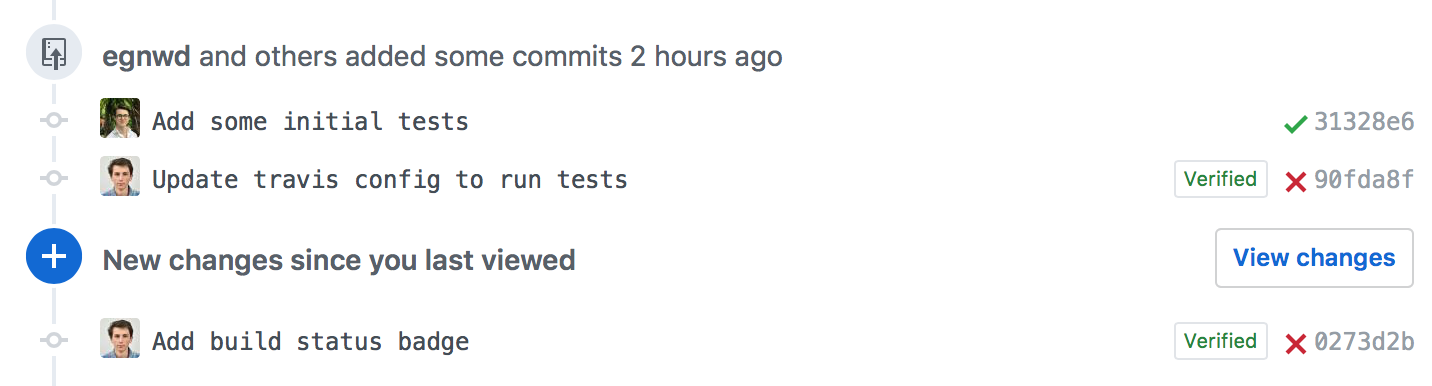
\includegraphics[width=\linewidth]{ci-1.png}
    \caption{Shows build status of commits within the code review}
    \label{fig:ci-1}
  \end{subfigure}
  \hfill
  \begin{subfigure}[h]{0.4\linewidth}
    \centering
    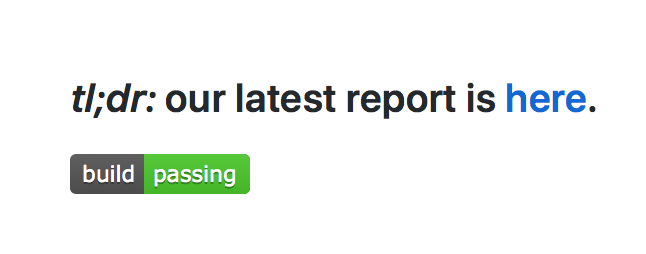
\includegraphics[width=\linewidth]{ci-2.png}
    \caption{Our git repo homepage shows us the current state of master}
    \label{fig:ci-2}
  \end{subfigure}
  \\
  \begin{subfigure}[h]{0.4\linewidth}
    \centering
    
\includegraphics[width=\linewidth]{ci-3.png}
    \caption{Tests help us avoid embarrassing mistakes, e.g.~the wrong title}
    \label{fig:ci-3}
  \end{subfigure}
  \hfill
  \begin{subfigure}[h]{0.4\linewidth}
    \centering
    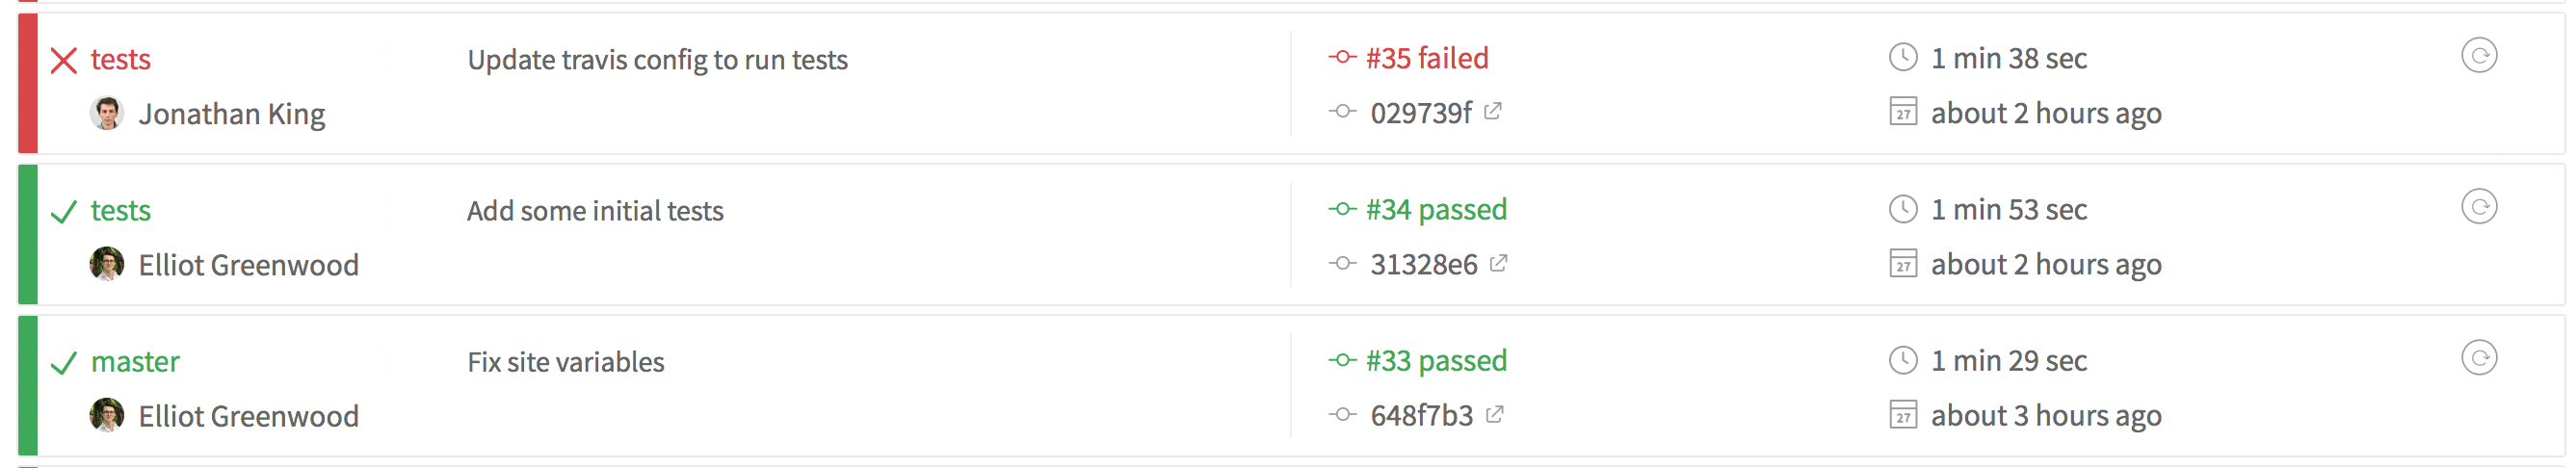
\includegraphics[width=\linewidth]{ci-4.png}
    \caption{Clear build log of builds and releases}
    \label{fig:ci-4}
  \end{subfigure}
  \\
  \begin{subfigure}[h]{0.4\linewidth}
    \centering
    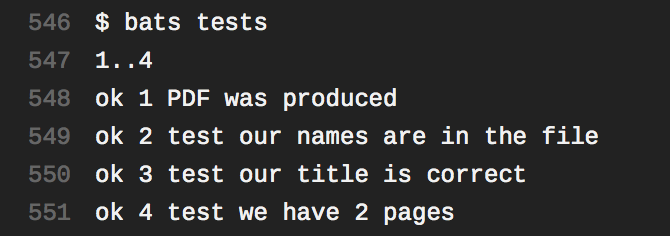
\includegraphics[width=\linewidth]{ci-5.png}
    \caption{Testing our report}
    \label{fig:ci-5}
  \end{subfigure}
  \caption{Screenshots of our build pipeline}
  \label{fig:}
\end{figure}

\begin{figure}[ht]
  \centering
  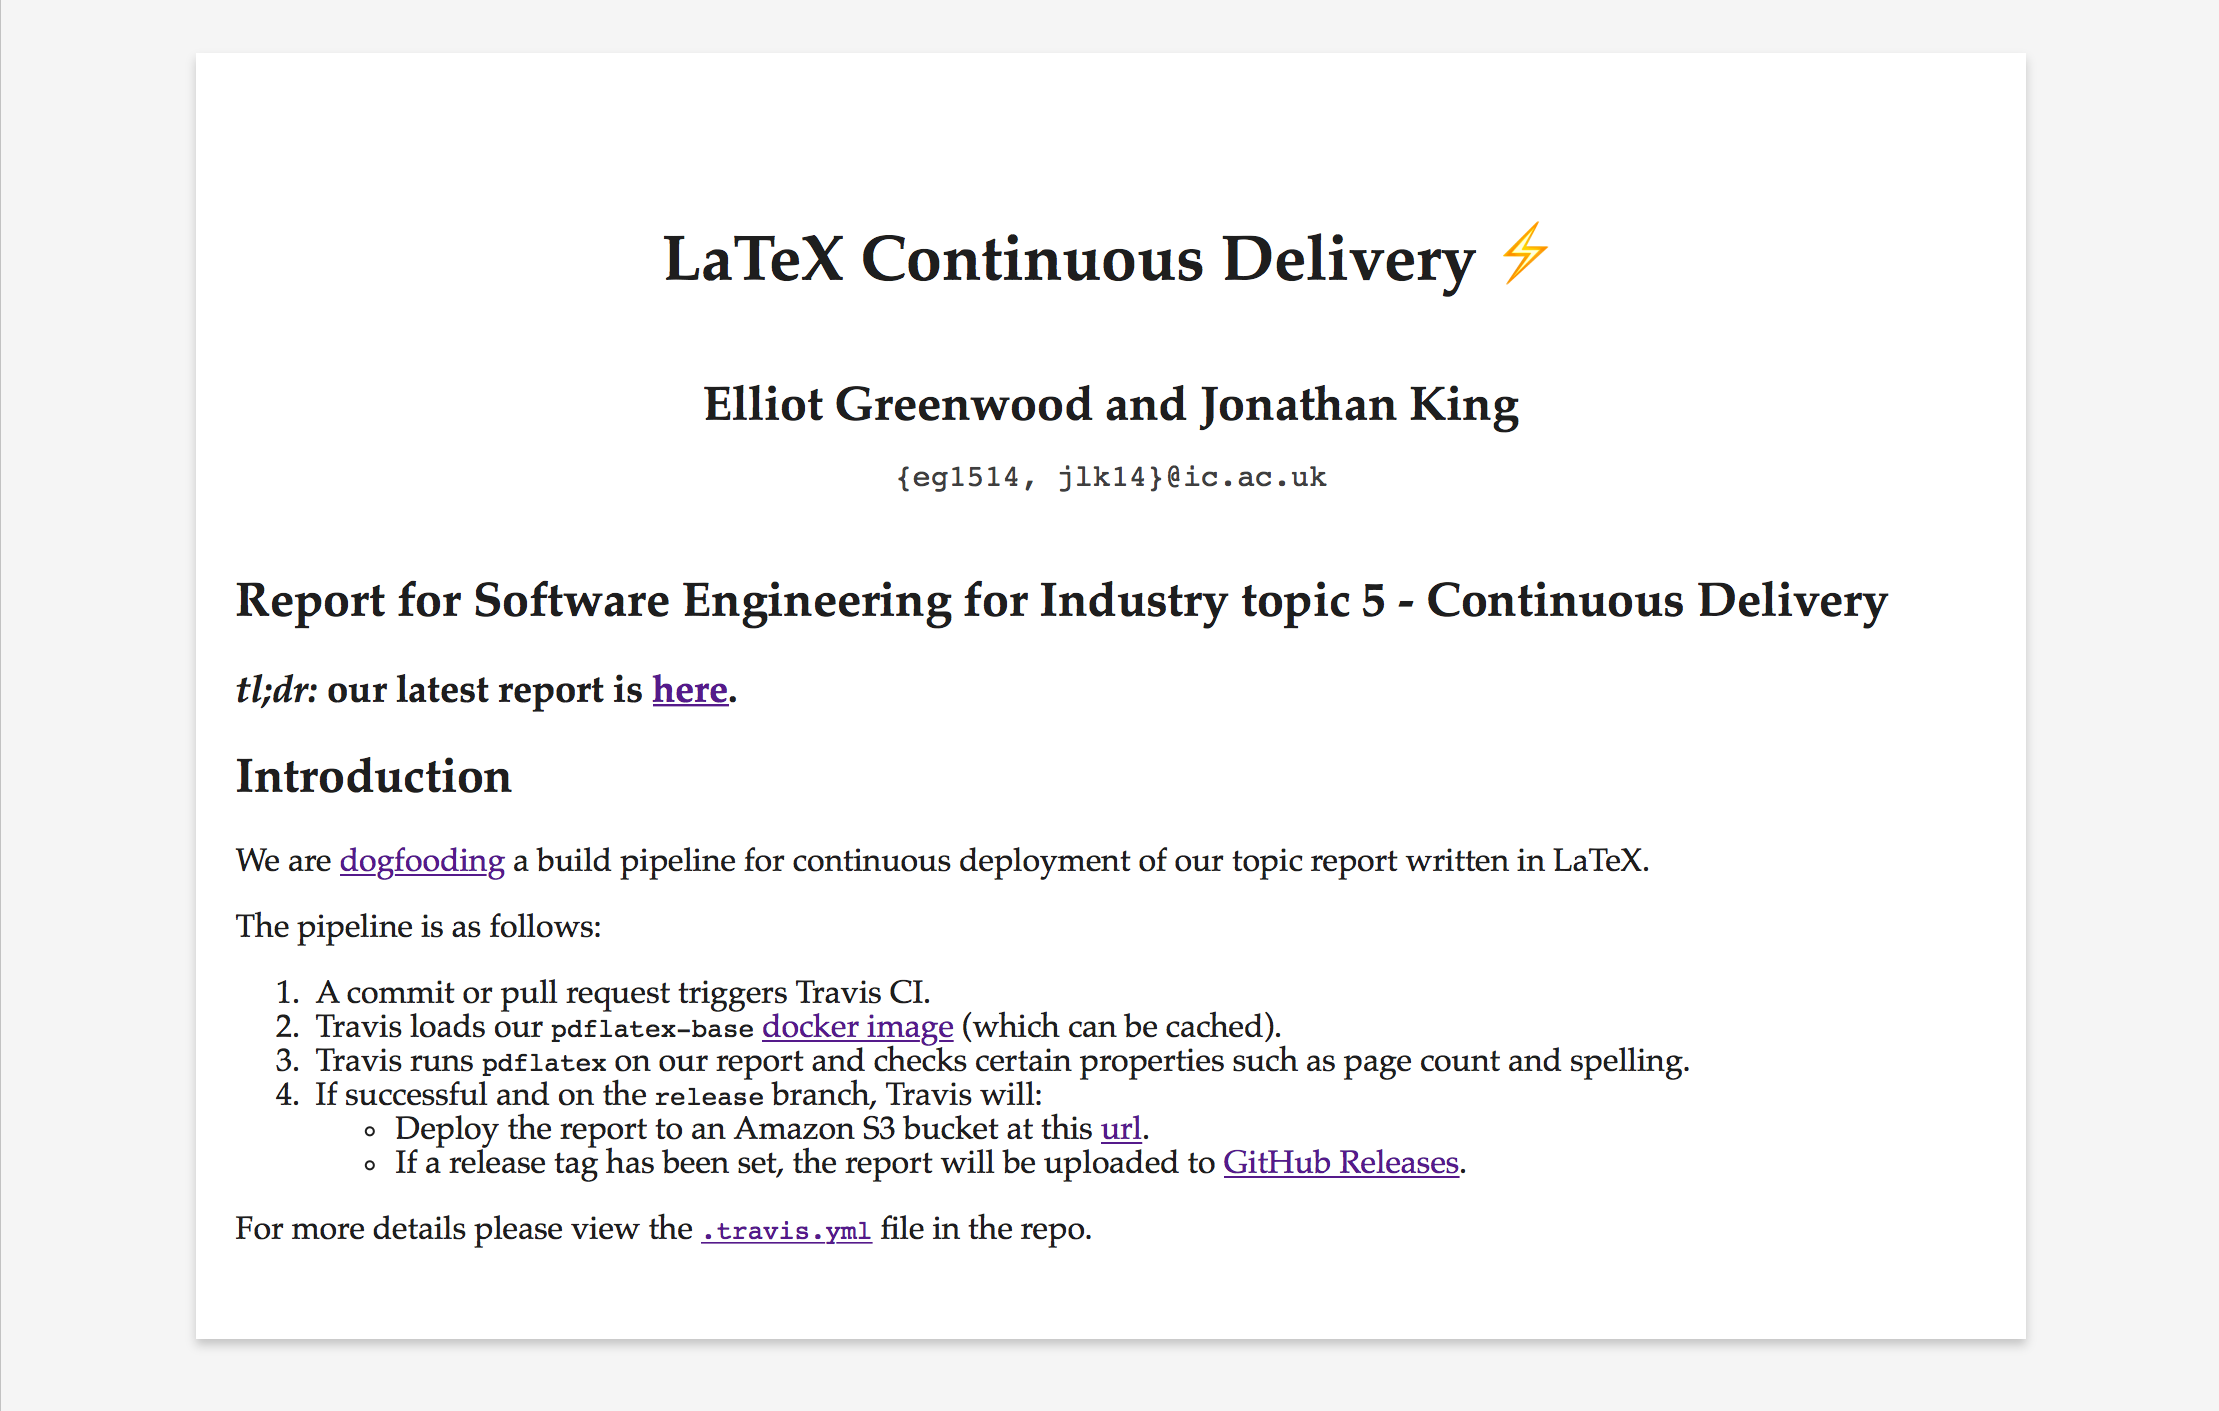
\includegraphics[width=0.7\linewidth]{ci-6.png}
  \caption{Screenshot of our project page}
  \label{fig:}
\end{figure}


\end{document}
